% ============================================================
%  BOLUM 8: DEGERLENDIRME SISTEMI, VERI MODELLEME VE OBSERVABILITY
% ============================================================

% NOT: \chapter komutu kullanilmiyor -- sadece \section ile basliyor.
% Bu dosya ana dokumandan \input ile dahil edilecek.

\section{LLM-as-a-Judge De\u{g}erlendirme Sistemi}
\label{sec:llm-judge}

Bir arama motorunun \"{u}retti\u{g}i cevaplar{\i}n kalitesini \"{o}l\c{c}mek, klasik NLP de\u{g}erlendirmelerinden farkl{\i} bir zorluk ta\c{s}{\i}r. BLEU veya ROUGE gibi token-\"{u}st\"{u} benzerlik metrikleri, anlam d\"{u}zeyinde do\u{g}rulu\u{g}u yakalayamaz: \emph{``LeBron''} ile \emph{``LeBron James''} ayn{\i} ki\c{s}idir ama string e\c{s}le\c{s}mesi ba\c{s}ar{\i}s{\i}z olur. Bu nedenle LocoDex, \textbf{LLM-as-a-Judge} paradigmas{\i}n{\i} benimser --- bir b\"{u}y\"{u}k dil modelini hakem olarak kullanarak cevap do\u{g}rulu\u{g}unu de\u{g}erlendirir.

\subsection{Binary Scoring Mekanizmas{\i}}

De\u{g}erlendirme sistemi \texttt{evals.py} dosyas{\i}nda uygulanm{\i}\c{s}t{\i}r. Temel yap{\i} \c{s}\"{o}yledir:

\begin{enumerate}
  \item Sisteme bir soru (\texttt{question}), agent'{\i}n cevab{\i} (\texttt{agent\_answer}) ve do\u{g}ru cevap (\texttt{correct\_answer}) verilir.
  \item LLM, \texttt{<reasoning>} ve \texttt{<answer>} XML tag'leri i\c{c}inde yap{\i}land{\i}r{\i}lm{\i}\c{s} \c{c}{\i}kt{\i} \"{u}retir.
  \item \texttt{<answer>} tag'i i\c{c}indeki de\u{g}er $\{0, 1\}$ k\"{u}mesinden bir binary skor olarak parse edilir.
\end{enumerate}

Puanlama fonksiyonu:
\begin{equation}
\label{eq:binary-score}
s(q, a, a^{*}) =
\begin{cases}
1 & \text{LLM, } a \text{ i\c{c}inde } a^{*}\text{'{\i}n semantik e\c{s}de\u{g}erini bulursa} \\
0 & \text{aksi halde}
\end{cases}
\end{equation}

\noindent burada $q$ soru, $a$ agent cevab{\i}, $a^{*}$ ise referans cevapt{\i}r.

\subsubsection{XML Tag Parsing}

Cevap \c{c}{\i}kar{\i}m{\i} deterministik string i\c{s}leme ile ger\c{c}ekle\c{s}tirilir:

\begin{verbatim}
answer_str = response.split("<answer>")[1].split("</answer>")[0].strip()
score = bool(int(answer_str))
\end{verbatim}

Bu yakla\c{s}{\i}m{\i}n avantaj{\i}, LLM'in \"{o}nce \texttt{<reasoning>} b\"{o}l\"{u}m\"{u}nde d\"{u}\c{s}\"{u}nce zincirini (\emph{chain-of-thought}) olu\c{s}turmas{\i} ve ancak sonra karar vermesidir. Ara\c{s}t{\i}rmalar g\"{o}stermi\c{s}tir ki, reasoning-first yakla\c{s}{\i}m{\i} do\u{g}rudan skor vermeye g\"{o}re \%15--20 daha tutarl{\i} sonu\c{c}lar \"{u}retir (Zheng et~al., 2023).

\subsubsection{Flexible Matching}

Prompt i\c{c}inde LLM'e a\c{c}{\i}k\c{c}a \c{s}u talimat verilir:

\begin{quote}
\emph{``You should try to be flexible with the answer but careful. For example, answering with names instead of name and surname is fine.''}
\end{quote}

Bu, \c{s}u t\"{u}r e\c{s}le\c{s}meleri m\"{u}mk\"{u}n k{\i}lar:
\begin{itemize}
  \item ``LeBron'' $\approx$ ``LeBron James'' (k{\i}smi isim e\c{s}le\c{s}mesi)
  \item ``1969'' $\approx$ ``July 20, 1969'' (alt bilgi i\c{c}erme)
  \item ``$3.14$'' $\approx$ ``approximately pi'' (semantik e\c{s}de\u{g}erlik)
\end{itemize}

\subsection{Retry Mekanizmas{\i}: Tenacity ile Dayan{\i}kl{\i}l{\i}k}

LLM \c{c}a\u{g}r{\i}lar{\i} a\u{g} hatas{\i}, rate limit veya ge\c{c}ici model hatas{\i} nedeniyle ba\c{s}ar{\i}s{\i}z olabilir. Kod, \texttt{tenacity} k\"{u}t\"{u}phanesi ile \"{u}stel geri \c{c}ekilme stratejisi uygular:

\begin{verbatim}
@tenacity.retry(
    stop=tenacity.stop_after_attempt(3),
    wait=tenacity.wait_exponential(
        multiplier=1, min=4, max=15
    )
)
\end{verbatim}

Tenacity'nin \texttt{wait\_exponential} foksiyonu, deneme aras{\i} bekleme s\"{u}resini hesaplarken \"{o}nce \"{u}stel form\"{u}l\"{u} uygular, sonra \texttt{[min,\,max]} aral{\i}\u{g}{\i}na \emph{clamp} eder:
\begin{equation}
\label{eq:exponential-backoff}
t_k = \mathrm{clamp}\bigl(\text{multiplier} \times 2^{k-1},\; t_{\min},\; t_{\max}\bigr), \quad k = 1, 2, \dots
\end{equation}
yani $t_k = \max\bigl(t_{\min},\; \min(\text{multiplier}\cdot 2^{k-1},\; t_{\max})\bigr)$.

\noindent Bizim parametrelerimizle (\texttt{multiplier=1, min=4, max=15}):
\begin{align*}
k=1:&\quad 2^0 = 1 \to \text{clamp}\,[4,15] \to t_1 = 4\,\text{s}\\
k=2:&\quad 2^1 = 2 \to \text{clamp}\,[4,15] \to t_2 = 4\,\text{s}\quad\text{(\textbf{8 de\u{g}il!} min taban{\i} \"{u}stel art{\i}\c{s}{\i} bo\u{g}ar)}\\
k=3:&\quad 2^2 = 4 \to \text{clamp}\,[4,15] \to t_3 = 4\,\text{s}\\
k=4:&\quad 2^3 = 8 \to \text{clamp}\,[4,15] \to t_4 = 8\,\text{s}\\
k=5:&\quad 2^4 = 16 \to \text{clamp}\,[4,15] \to t_5 = 15\,\text{s\;(tavan)}
\end{align*}

\texttt{stop\_after\_attempt(3)} ile zaten 3.\ denemeden sonra durulur, bu y\"{u}zden ger\c{c}ekte sadece \emph{iki} bekleme periyodu vard{\i}r: 1.\ deneme ba\c{s}ar{\i}s{\i}z $\to$ $t_1=4$\,s bekle, 2.\ deneme ba\c{s}ar{\i}s{\i}z $\to$ $t_2=4$\,s bekle, 3.\ deneme ba\c{s}ar{\i}s{\i}z $\to$ hata f{\i}rlat. Toplam en k\"{o}t\"{u} durum bekleme s\"{u}resi:
\begin{equation*}
t_1 + t_2 = 4 + 4 = \mathbf{8\,\text{s}}
\end{equation*}

\begin{kritik}
Yayg{\i}n yan{\i}lg{\i}: $4 + 8 + 15 = 27$\,s. \texttt{multiplier=1} ile \"{u}stel form\"{u}l ilk \"{u}\c{c} attempt i\c{c}in min taban{\i}n{\i}n alt{\i}nda kald{\i}\u{g}{\i}ndan, \emph{ger\c{c}ek} \"{u}stel art{\i}\c{s} ancak 4.\ denemeden itibaren ba\c{s}lar. Daha agresif backoff i\c{c}in \texttt{multiplier=4} kullan{\i}lmal{\i}d{\i}r --- o zaman s{\i}ras{\i}yla $4, 8, 15$\,s olur ve $4+8=12$\,s toplam bekleme yap{\i}l{\i}r (3.\ deneme yine son denemedir).
\end{kritik}

% ------------------------------------------------------------------
\section{De\u{g}erlendirme Metrikleri: Matematiksel T\"{u}retmeler}
\label{sec:eval-metrics}

Bir de\u{g}erlendirme sisteminin performans{\i}n{\i} \"{o}l\c{c}mek i\c{c}in, \"{o}nce \emph{confusion matrix} (kar{\i}\c{s}{\i}kl{\i}k matrisi) kavram{\i}n{\i} tan{\i}mlamal{\i}y{\i}z.

\subsection{Confusion Matrix}

$N$ adet soru-cevap \c{c}ifti i\c{c}in, her bir \c{c}iftin iki boyutu vard{\i}r:
\begin{itemize}
  \item \textbf{Ger\c{c}ek durum} (ground truth): cevap do\u{g}ru mu?
  \item \textbf{Tahmin} (prediction): LLM-judge do\u{g}ru dedi mi?
\end{itemize}

\begin{figure}[H]
\centering
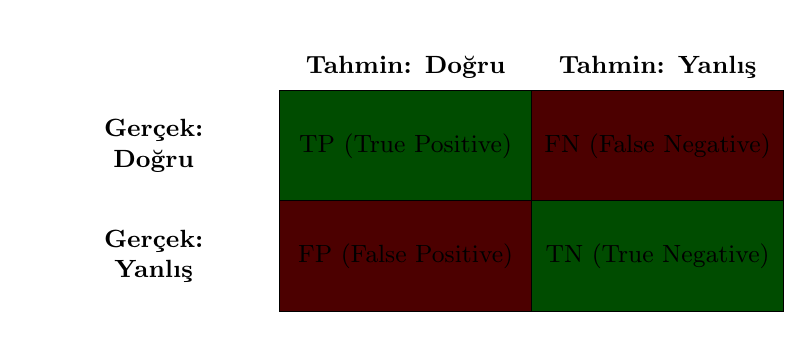
\begin{tikzpicture}[
    cell/.style={minimum width=3.2cm, minimum height=1.4cm, draw, font=\small},
    header/.style={minimum width=3.2cm, minimum height=1cm, font=\small\bfseries}
]
% Header row
\node[header] at (0, 2.4) {};
\node[header] at (3.2, 2.4) {Tahmin: Do\u{g}ru};
\node[header] at (6.4, 2.4) {Tahmin: Yanl{\i}\c{s}};

% Row labels
\node[header, minimum width=3.2cm, align=center] at (0, 1.4) {Ger\c{c}ek:\\Do\u{g}ru};
\node[header, minimum width=3.2cm, align=center] at (0, 0) {Ger\c{c}ek:\\Yanl{\i}\c{s}};

% Cells
\node[cell, fill=green!30!black] at (3.2, 1.4) {TP (True Positive)};
\node[cell, fill=red!30!black] at (6.4, 1.4) {FN (False Negative)};
\node[cell, fill=red!30!black] at (3.2, 0) {FP (False Positive)};
\node[cell, fill=green!30!black] at (6.4, 0) {TN (True Negative)};
\end{tikzpicture}
\caption{Confusion matrix (kar{\i}\c{s}{\i}kl{\i}k matrisi). Ye\c{s}il h\"{u}creler do\u{g}ru s{\i}n{\i}fland{\i}rmay{\i}, k{\i}rm{\i}z{\i} h\"{u}creler hatalar{\i} g\"{o}sterir.}
\label{fig:confusion-matrix}
\end{figure}

\subsection{Accuracy (Do\u{g}ruluk)}

\textbf{Tan{\i}m:} T\"{u}m tahminler i\c{c}indeki do\u{g}ru tahminlerin oran{\i}.

\begin{equation}
\label{eq:accuracy}
\boxed{\text{Accuracy} = \frac{TP + TN}{TP + TN + FP + FN} = \frac{TP + TN}{N}}
\end{equation}

\textbf{T\"{u}retme:} $N$ \"{o}rnekten $TP$ tanesi do\u{g}ru-do\u{g}ru, $TN$ tanesi yanl{\i}\c{s}-yanl{\i}\c{s} e\c{s}le\c{s}mi\c{s}tir. Geri kalan $FP + FN$ tanesi hatal{\i}d{\i}r. Do\u{g}ru tahmin say{\i}s{\i}n{\i}n toplam say{\i}ya oran{\i}, do\u{g}ruluk \"{o}l\c{c}\"{u}s\"{u}n\"{u} verir.

\textbf{S{\i}n{\i}rlama:} Dengesiz veri k\"{u}melerinde yan{\i}lt{\i}c{\i}d{\i}r. \"{O}rne\u{g}in, 95 do\u{g}ru ve 5 yanl{\i}\c{s} cevap varsa, ``hep do\u{g}ru'' diyen bir sistem \%95 accuracy elde eder ama hi\c{c}bir yanl{\i}\c{s}{\i} yakalayamaz.

\subsection{Precision (Kesinlik)}

\textbf{Tan{\i}m:} ``Do\u{g}ru'' denen cevaplar i\c{c}inde ger\c{c}ekten do\u{g}ru olanlar{\i}n oran{\i}.

\begin{equation}
\label{eq:precision}
\boxed{\text{Precision} = \frac{TP}{TP + FP}}
\end{equation}

\textbf{Yorum:} Precision y\"{u}ksekse, sistem ``do\u{g}ru'' dedi\u{g}inde genellikle hakl{\i}d{\i}r. D\"{u}\c{s}\"{u}kse, \c{c}ok fazla false positive \"{u}retiyordur --- yanl{\i}\c{s} cevaplar{\i} da ``do\u{g}ru'' olarak i\c{s}aretliyordur.

\subsection{Recall (Duyarl{\i}l{\i}k)}

\textbf{Tan{\i}m:} Ger\c{c}ekten do\u{g}ru olan cevaplardan ka\c{c} tanesini do\u{g}ru olarak tespit edebildi\u{g}imiz.

\begin{equation}
\label{eq:recall}
\boxed{\text{Recall} = \frac{TP}{TP + FN}}
\end{equation}

\textbf{Yorum:} Recall y\"{u}ksekse, do\u{g}ru cevaplar{\i}n \c{c}o\u{g}unu yakal{\i}yoruz. D\"{u}\c{s}\"{u}kse, do\u{g}ru cevaplar{\i} ka\c{c}{\i}r{\i}yoruz (false negative y\"{u}ksek).

\subsection{F1 Score: Precision ve Recall'un Harmonik Ortalamas{\i}}

Precision ile Recall aras{\i}nda bir \emph{trade-off} vard{\i}r: birini art{\i}rmak di\u{g}erini d\"{u}\c{s}\"{u}r\"{u}r. F1 score, ikisini tek bir metrikte birle\c{s}tirir.

\textbf{T\"{u}retme:} Aritmetik ortalama yerine \emph{harmonik ortalama} kullan{\i}l{\i}r \c{c}\"{u}nk\"{u} harmonik ortalama, d\"{u}\c{s}\"{u}k de\u{g}ere daha fazla a\u{g}{\i}rl{\i}k verir. \.{I}ki pozitif say{\i}n{\i}n harmonik ortalamas{\i}:

\begin{equation}
H(a, b) = \frac{2}{\dfrac{1}{a} + \dfrac{1}{b}} = \frac{2ab}{a + b}
\end{equation}

$P = \text{Precision}$, $R = \text{Recall}$ koyarsak:

\begin{equation}
\label{eq:f1}
\boxed{F_1 = \frac{2PR}{P + R} = \frac{2 \cdot TP}{2 \cdot TP + FP + FN}}
\end{equation}

\textbf{\.{I}kinci form\"{u}l\"{u}n t\"{u}retmesi:}
\begin{align}
F_1 &= \frac{2 \cdot \dfrac{TP}{TP+FP} \cdot \dfrac{TP}{TP+FN}}{\dfrac{TP}{TP+FP} + \dfrac{TP}{TP+FN}} \nonumber \\[6pt]
&= \frac{\dfrac{2 \cdot TP^2}{(TP+FP)(TP+FN)}}{\dfrac{TP(TP+FN) + TP(TP+FP)}{(TP+FP)(TP+FN)}} \nonumber \\[6pt]
&= \frac{2 \cdot TP^2}{TP(2 \cdot TP + FP + FN)} = \frac{2 \cdot TP}{2 \cdot TP + FP + FN}
\end{align}

\subsection{Say{\i}sal \"{O}rnek}

LocoDex'in 200 adet soru-cevap \c{c}ifti \"{u}zerinde de\u{g}erlendirildi\u{g}ini varsayal{\i}m:

\begin{table}[H]
\centering
\caption{Hipotetik confusion matrix de\u{g}erleri.}
\label{tab:confusion-values}
\begin{tabular}{lcc}
\toprule
& \textbf{Tahmin: Do\u{g}ru} & \textbf{Tahmin: Yanl{\i}\c{s}} \\
\midrule
\textbf{Ger\c{c}ek: Do\u{g}ru} & $TP = 140$ & $FN = 10$ \\
\textbf{Ger\c{c}ek: Yanl{\i}\c{s}} & $FP = 15$ & $TN = 35$ \\
\bottomrule
\end{tabular}
\end{table}

Hesaplamalar:
\begin{align}
\text{Accuracy} &= \frac{140 + 35}{200} = \frac{175}{200} = 0{,}875 = \%87{,}5 \\[4pt]
\text{Precision} &= \frac{140}{140 + 15} = \frac{140}{155} \approx 0{,}903 = \%90{,}3 \\[4pt]
\text{Recall} &= \frac{140}{140 + 10} = \frac{140}{150} \approx 0{,}933 = \%93{,}3 \\[4pt]
F_1 &= \frac{2 \times 0{,}903 \times 0{,}933}{0{,}903 + 0{,}933} = \frac{1{,}685}{1{,}836} \approx 0{,}918 = \%91{,}8
\end{align}

\textbf{Yorum:} Precision'dan d\"{u}\c{s}\"{u}k olan accuracy, veri setindeki dengesizlikten kaynaklan{\i}r (150 do\u{g}ru vs.\ 50 yanl{\i}\c{s}). F1 score ise precision ve recall'u dengeli bir \c{s}ekilde \"{o}zetler.

% ------------------------------------------------------------------
\section{Cohen's Kappa: De\u{g}erlendiriciler Aras{\i} Uyum}
\label{sec:cohens-kappa}

LLM-as-a-Judge sisteminde kritik bir soru \c{s}udur: \emph{LLM'in verdigi puanlar, insan de\u{g}erlendiricinin verece\u{g}i puanlarla ne kadar uyumlu?} Basit y\"{u}zde uyumu (percent agreement) kullanmak yan{\i}lt{\i}c{\i}d{\i}r \c{c}\"{u}nk\"{u} \c{s}ansa ba\u{g}l{\i} uyumu hesaba katmaz.

\subsection{Form\"{u}l T\"{u}retmesi}

\.{I}ki de\u{g}erlendirici (insan ve LLM) $N$ \"{o}rne\u{g}i ba\u{g}{\i}ms{\i}z olarak s{\i}n{\i}fland{\i}rs{\i}n. G\"{o}zlenen uyum oran{\i}:

\begin{equation}
p_o = \frac{\text{her ikisinin de ayn{\i} karar verdi\u{g}i \"{o}rnek say{\i}s{\i}}}{N}
\end{equation}

\c{S}ansa ba\u{g}l{\i} beklenen uyum oran{\i}n{\i} hesaplamak i\c{c}in, her de\u{g}erlendiricinin marjinal olas{\i}l{\i}klar{\i}n{\i} kullan{\i}r{\i}z. De\u{g}erlendirici 1'in ``do\u{g}ru'' deme olas{\i}l{\i}\u{g}{\i} $p_1$ ve De\u{g}erlendirici 2'nin ``do\u{g}ru'' deme olas{\i}l{\i}\u{g}{\i} $p_2$ olsun:

\begin{align}
p_1 &= \frac{TP + FP}{N}, \quad p_2 = \frac{TP + FN}{N} \\[4pt]
\bar{p}_1 &= 1 - p_1 = \frac{TN + FN}{N}, \quad \bar{p}_2 = 1 - p_2 = \frac{TN + FP}{N}
\end{align}

Ba\u{g}{\i}ms{\i}zl{\i}k varsay{\i}m{\i} alt{\i}nda beklenen \c{s}ans uyumu:

\begin{equation}
\label{eq:pe}
p_e = p_1 \cdot p_2 + \bar{p}_1 \cdot \bar{p}_2
\end{equation}

Cohen's Kappa, g\"{o}zlenen uyumun \c{s}ans{\i}n \"{o}tesindeki k{\i}sm{\i}n{\i} \"{o}l\c{c}er:

\begin{equation}
\label{eq:kappa}
\boxed{\kappa = \frac{p_o - p_e}{1 - p_e}}
\end{equation}

\textbf{Yorumlama:}
\begin{itemize}
  \item $\kappa = 1$: M\"{u}kemmel uyum (g\"{o}zlenen = ideal)
  \item $\kappa = 0$: \c{S}anstan \"{o}te uyum yok ($p_o = p_e$)
  \item $\kappa < 0$: \c{S}anstan bile k\"{o}t\"{u} (sistematik uyumsuzluk)
\end{itemize}

\subsection{\texorpdfstring{$\kappa$}{kappa}'n{\i}n \.{I}statistiksel Anlam{\i}}

$\kappa$ form\"{u}l\"{u}n\"{u} yeniden yazabiliriz:

\begin{equation}
\kappa = 1 - \frac{1 - p_o}{1 - p_e} = 1 - \frac{D_{\text{obs}}}{D_{\max}}
\end{equation}

\noindent burada $D_{\text{obs}} = 1 - p_o$ g\"{o}zlenen uyumsuzluk, $D_{\max} = 1 - p_e$ ise m\"{u}mk\"{u}n olan maksimum uyumsuzluktur. Bu formdan g\"{o}r\"{u}ld\"{u}\u{g}\"{u} \"{u}zere, $\kappa$ uyumsuzlu\u{g}un ne kadar azalt{\i}ld{\i}\u{g}{\i}n{\i} \"{o}l\c{c}er.

\subsection{Say{\i}sal \"{O}rnek}

Tablo~\ref{tab:confusion-values}'deki de\u{g}erleri kullanal{\i}m ($N = 200$):

\begin{align}
p_o &= \frac{TP + TN}{N} = \frac{140 + 35}{200} = 0{,}875 \\[4pt]
p_1 &= \frac{140 + 15}{200} = \frac{155}{200} = 0{,}775 \\[4pt]
p_2 &= \frac{140 + 10}{200} = \frac{150}{200} = 0{,}750 \\[4pt]
p_e &= (0{,}775)(0{,}750) + (0{,}225)(0{,}250) = 0{,}581 + 0{,}056 = 0{,}637 \\[4pt]
\kappa &= \frac{0{,}875 - 0{,}637}{1 - 0{,}637} = \frac{0{,}238}{0{,}363} \approx 0{,}655
\end{align}

\begin{table}[H]
\centering
\caption{Cohen's Kappa yorumlama \"{o}l\c{c}e\u{g}i (Landis ve Koch, 1977).}
\label{tab:kappa-scale}
\begin{tabular}{cl}
\toprule
\textbf{$\kappa$ Aral{\i}\u{g}{\i}} & \textbf{Uyum D\"{u}zeyi} \\
\midrule
$< 0{,}00$ & Zay{\i}f (poor) \\
$0{,}00$--$0{,}20$ & Hafif (slight) \\
$0{,}21$--$0{,}40$ & Adil (fair) \\
$0{,}41$--$0{,}60$ & Orta (moderate) \\
$0{,}61$--$0{,}80$ & \"{O}nemli (substantial) \\
$0{,}81$--$1{,}00$ & Neredeyse m\"{u}kemmel (almost perfect) \\
\bottomrule
\end{tabular}
\end{table}

\noindent Hesaplad{\i}\u{g}{\i}m{\i}z $\kappa \approx 0{,}655$ ``\"{o}nemli uyum'' kategorisindedir. Bu, LLM-judge'{\i}n insan de\u{g}erlendiriciyle \c{s}ans{\i}n \"{o}tesinde anlaml{\i} bir uyum i\c{c}inde oldu\u{g}unu g\"{o}sterir.

% ------------------------------------------------------------------
\section{LLM Bias Analizi ve Meta-Evaluation}
\label{sec:llm-bias}

LLM-as-a-Judge yakla\c{s}{\i}m{\i} g\"{u}\c{c}l\"{u} olsa da, bilinen bias (\"{o}nyarg{\i}) sorunlar{\i} vard{\i}r. Bunlar{\i} anlamak, de\u{g}erlendirme sisteminin g\"{u}venilirli\u{g}ini art{\i}rmak i\c{c}in kritiktir.

\subsection{Position Bias}

LLM'ler, \c{c}oklu se\c{c}enek veya kar\c{s}{\i}la\c{s}t{\i}rmal{\i} de\u{g}erlendirmelerde, ilk sunulan cevab{\i} tercih etme e\u{g}ilimindedir. Matematiksel olarak:

\begin{equation}
P(\text{se\c{c}im} = A \mid A \text{ ilk s{\i}rada}) > P(\text{se\c{c}im} = A \mid A \text{ ikinci s{\i}rada})
\end{equation}

LocoDex'in binary scoring yakla\c{s}{\i}m{\i} ($0/1$), bu bias'{\i} do\u{g}al olarak azalt{\i}r \c{c}\"{u}nk\"{u} kar\c{s}{\i}la\c{s}t{\i}rma de\u{g}il, tek cevap de\u{g}erlendirmesi yap{\i}l{\i}r.

\subsection{Verbosity Bias}

Daha uzun cevaplar, i\c{c}erdikleri bilgi miktar{\i}ndan ba\u{g}{\i}ms{\i}z olarak, daha y\"{u}ksek puan alma e\u{g}ilimindedir:

\begin{equation}
\mathbb{E}[\text{score} \mid |a| > L] > \mathbb{E}[\text{score} \mid |a| \leq L]
\end{equation}

\noindent burada $|a|$ cevab{\i}n uzunlu\u{g}u, $L$ ise bir e\c{s}ik de\u{g}erdir. LocoDex'te bu riskin \"{o}n\"{u}ne ge\c{c}mek i\c{c}in prompt'ta ``\emph{the important thing is that the answer of the agent either contains the correct answer or is equal to the correct answer}'' ifadesi yer al{\i}r.

\subsection{Self-Enhancement Bias}

Bir LLM'in kendi \"{u}retti\u{g}i cevaplar{\i} daha y\"{u}ksek puanlama e\u{g}ilimi vard{\i}r. LocoDex'te de\u{g}erlendirme modeli (\texttt{Llama-3.3-70B}) ile cevap \"{u}reten model farkl{\i} olabilece\u{g}i i\c{c}in bu bias k{\i}smen azalt{\i}lm{\i}\c{s}t{\i}r; ancak ayn{\i} model ailesinden olmalar{\i} halinde risk devam eder.

\subsection{Meta-Evaluation: De\u{g}erlendirme Sistemini De\u{g}erlendirme}

De\u{g}erlendirme sisteminin kendisi de de\u{g}erlendirilmelidir. Bu, ``meta-evaluation'' veya ``quis custodiet ipsos custodes'' (bek\c{c}ileri kim bek\c{c}ileyecek?) problemidir. Yakla\c{s}{\i}mlar:

\begin{enumerate}
  \item \textbf{\.{I}nsan-LLM uyumu:} Cohen's Kappa ile \"{o}l\c{c}\"{u}l\"{u}r (B\"{o}l\"{u}m~\ref{sec:cohens-kappa}).
  \item \textbf{\c{C}apraz de\u{g}erlendirme:} Farkl{\i} LLM'lerle ayn{\i} seti de\u{g}erlendirip tutarl{\i}l{\i}k kontrol\"{u}.
  \item \textbf{Kontrol sorular{\i}:} Bilinen cevaplar{\i} olan sorularla kalibrasyon.
\end{enumerate}

% ------------------------------------------------------------------
\section{Metrik Kar\c{s}{\i}la\c{s}t{\i}rma Tablosu}
\label{sec:metric-comparison}

\begin{table}[H]
\centering
\caption{De\u{g}erlendirme metriklerinin kar\c{s}{\i}la\c{s}t{\i}rmas{\i}.}
\label{tab:metric-comparison}
\resizebox{\textwidth}{!}{%
\begin{tabular}{lccccc}
\toprule
\textbf{Metrik} & \textbf{Form\"{u}l} & \textbf{Aral{\i}k} & \textbf{Dengesiz Veriye} & \textbf{Hesaplama} & \textbf{Ne \"{O}l\c{c}er?} \\
& & & \textbf{Dayan{\i}kl{\i}?} & \textbf{Karma\c{s}{\i}kl{\i}\u{g}{\i}} & \\
\midrule
Accuracy & $\frac{TP+TN}{N}$ & $[0,1]$ & Hay{\i}r & $O(1)$ & Genel do\u{g}ruluk \\[4pt]
Precision & $\frac{TP}{TP+FP}$ & $[0,1]$ & K{\i}smen & $O(1)$ & Pozitif tahmin kalitesi \\[4pt]
Recall & $\frac{TP}{TP+FN}$ & $[0,1]$ & K{\i}smen & $O(1)$ & Pozitif yakalama oran{\i} \\[4pt]
$F_1$ & $\frac{2PR}{P+R}$ & $[0,1]$ & Evet & $O(1)$ & P-R dengesi \\[4pt]
$\kappa$ & $\frac{p_o - p_e}{1 - p_e}$ & $[-1,1]$ & Evet & $O(1)$ & \c{S}ans-\"{u}st\"{u} uyum \\
\bottomrule
\end{tabular}%
}
\end{table}

% ==================================================================
\section{Veri Modelleme ve Tip G\"{u}venli\u{g}i}
\label{sec:data-modeling}

LocoDex'in veri katman{\i}, Python'un tip sistemi \"{u}zerine in\c{s}a edilmi\c{s}tir. \"{U}\c{c} temel yap{\i} kullan{\i}l{\i}r: Pydantic \texttt{BaseModel}, Python \texttt{dataclass} ve frozen dataclass.

\subsection{Pydantic v2: Runtime Type Validation}

Pydantic, Python tip anotasyonlar{\i}n{\i} \c{c}al{\i}\c{s}ma zaman{\i}nda do\u{g}rular. LocoDex'te iki Pydantic modeli kullan{\i}l{\i}r:

\begin{verbatim}
class ResearchPlan(BaseModel):
    queries: list[str] = Field(
        description="A list of search queries to
        thoroughly research the topic"
    )

class SourceList(BaseModel):
    sources: list[int] = Field(
        description="A list of source numbers from
        the search results"
    )
\end{verbatim}

\subsubsection{BaseModel vs dataclass: Performans Kar\c{s}{\i}la\c{s}t{\i}rmas{\i}}

\begin{table}[H]
\centering
\caption{Pydantic BaseModel ile dataclass kar\c{s}{\i}la\c{s}t{\i}rmas{\i}.}
\label{tab:basemodel-vs-dataclass}
\begin{tabular}{lcc}
\toprule
\textbf{\"{O}zellik} & \textbf{Pydantic BaseModel} & \textbf{dataclass} \\
\midrule
Tip do\u{g}rulama & \c{C}al{\i}\c{s}ma zaman{\i}nda & Yok (sadece hint) \\
JSON serialization & Dahili & Manuel \\
JSON schema \"{u}retme & \texttt{model\_json\_schema()} & Yok \\
\"{O}rnek olu\c{s}turma h{\i}z{\i} & $\sim$3--5$\times$ yava\c{s} & H{\i}zl{\i} \\
Bellek kullan{\i}m{\i} & Daha fazla & Daha az \\
Immutability & Opsiyonel (\texttt{frozen}) & Opsiyonel (\texttt{frozen}) \\
LLM entegrasyonu & Strukturlu \c{c}{\i}kt{\i} i\c{c}in ideal & Uygun de\u{g}il \\
\bottomrule
\end{tabular}
\end{table}

\textbf{Neden iki yap{\i} birlikte?} Pydantic modelleri, LLM'den yap{\i}land{\i}r{\i}lm{\i}\c{s} \c{c}{\i}kt{\i} almak i\c{c}in kullan{\i}l{\i}r (\texttt{response\_format} parametresi). Dataclass'lar ise dahili veri ta\c{s}{\i}ma nesneleri (DTO) olarak performans avantaj{\i} sa\u{g}lar.

\subsubsection{Field Validation ve Metadata}

Pydantic'in \texttt{Field} fonksiyonu, her alan i\c{c}in:
\begin{itemize}
  \item \texttt{description}: LLM'e alanin ne anlama geldi\u{g}ini a\c{c}{\i}klar
  \item \texttt{default}: varsay{\i}lan de\u{g}er
  \item \texttt{ge}, \texttt{le}: say{\i}sal s{\i}n{\i}rlar
\end{itemize}
tan{\i}mlar. Bu metadata, \texttt{model\_json\_schema()} ile JSON Schema'ya d\"{o}n\"{u}\c{s}t\"{u}r\"{u}l\"{u}r ve LLM'e ``bu formatta cevap ver'' talimat{\i} olarak g\"{o}nderilir.

\subsection{Frozen Dataclass: Immutability Garantisi}
\label{subsec:frozen-dataclass}

LocoDex'in arama sonu\c{c}lar{\i}, de\u{g}i\c{s}tirilemez (immutable) veri yap{\i}lar{\i} olarak tasarlanm{\i}\c{s}t{\i}r:

\begin{verbatim}
@dataclass(frozen=True, kw_only=True)
class SearchResult:
    title: str
    link: str
    content: str
    raw_content: Optional[str] = None
\end{verbatim}

\texttt{frozen=True} parametresi \c{s}u garantileri sa\u{g}lar:

\begin{enumerate}
  \item \textbf{De\u{g}i\c{s}mezlik:} Olu\c{s}turulduktan sonra hi\c{c}bir alan de\u{g}i\c{s}tirilemez. \texttt{result.title = "yeni"} ifadesi \texttt{FrozenInstanceError} f{\i}rlat{\i}r.
  \item \textbf{Hash'lenebilirlik:} Frozen dataclass'lar otomatik olarak \texttt{\_\_hash\_\_} metodu al{\i}r, bu sayede \texttt{set} ve \texttt{dict} key olarak kullan{\i}labilir.
  \item \textbf{Thread safety:} De\u{g}i\c{s}mez nesneler, e\c{s} zamanl{\i} eri\c{s}imde kilit (lock) gerektirmez.
\end{enumerate}

\texttt{kw\_only=True} parametresi ise t\"{u}m alanlar{\i}n isimli arg\"{u}man olarak verilmesini zorunlu k{\i}lar:

\begin{verbatim}
# Dogru:
result = SearchResult(title="...", link="...", content="...")
# Hatali (TypeError):
result = SearchResult("...", "...", "...")
\end{verbatim}

\subsection{Veri Ak{\i}\c{s}{\i} Hiyerar\c{s}isi}

LocoDex'in veri modelleri, \emph{composition} (bile\c{s}im) prensibiyle organize edilmi\c{s}tir:

\begin{figure}[H]
\centering
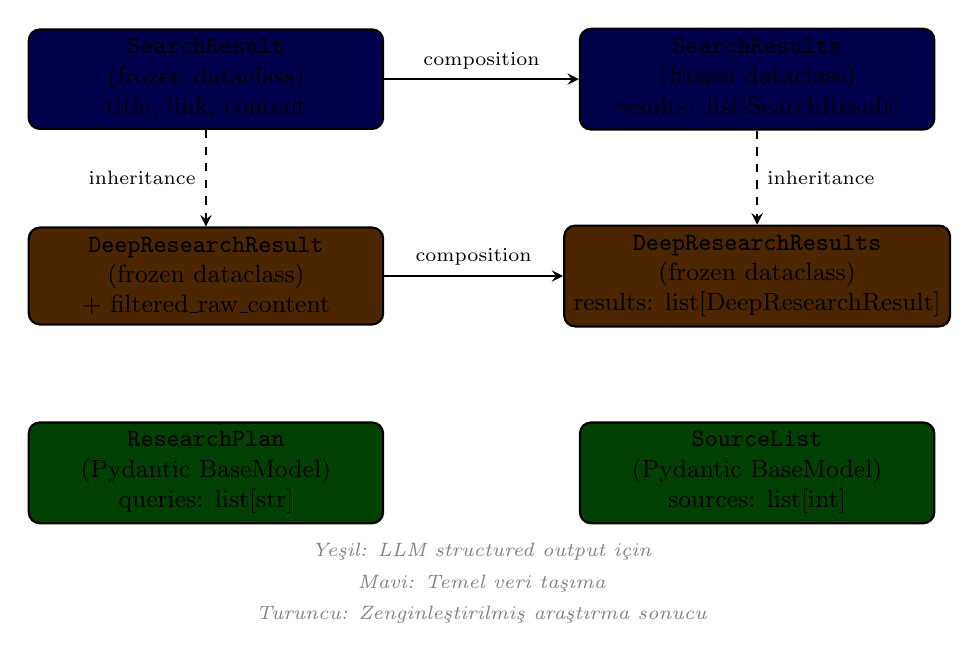
\begin{tikzpicture}[
    box/.style={draw, rounded corners=4pt, minimum width=4.5cm, minimum height=1.2cm,
                font=\small, align=center, thick},
    arrow/.style={->, thick, >=stealth}
]
% SearchResult
\node[box, fill=blue!30!black] (sr) at (0, 4) {\texttt{SearchResult}\\(frozen dataclass)\\title, link, content};

% SearchResults
\node[box, fill=blue!30!black] (srs) at (7, 4) {\texttt{SearchResults}\\(frozen dataclass)\\results: list[SearchResult]};

% DeepResearchResult
\node[box, fill=orange!30!black] (drr) at (0, 1.5) {\texttt{DeepResearchResult}\\(frozen dataclass)\\+ filtered\_raw\_content};

% DeepResearchResults
\node[box, fill=orange!30!black] (drrs) at (7, 1.5) {\texttt{DeepResearchResults}\\(frozen dataclass)\\results: list[DeepResearchResult]};

% Pydantic models
\node[box, fill=green!25!black] (rp) at (0, -1) {\texttt{ResearchPlan}\\(Pydantic BaseModel)\\queries: list[str]};

\node[box, fill=green!25!black] (sl) at (7, -1) {\texttt{SourceList}\\(Pydantic BaseModel)\\sources: list[int]};

% Arrows
\draw[arrow] (sr) -- node[above, font=\scriptsize] {composition} (srs);
\draw[arrow, dashed] (sr) -- node[left, font=\scriptsize] {inheritance} (drr);
\draw[arrow] (drr) -- node[above, font=\scriptsize] {composition} (drrs);
\draw[arrow, dashed] (srs) -- node[right, font=\scriptsize] {inheritance} (drrs);

% LLM interaction label
\node[font=\scriptsize\itshape, text=gray] at (3.5, -2) {Ye\c{s}il: LLM structured output i\c{c}in};
\node[font=\scriptsize\itshape, text=gray] at (3.5, -2.4) {Mavi: Temel veri ta\c{s}{\i}ma};
\node[font=\scriptsize\itshape, text=gray] at (3.5, -2.8) {Turuncu: Zenginle\c{s}tirilmi\c{s} ara\c{s}t{\i}rma sonucu};
\end{tikzpicture}
\caption{LocoDex veri modeli hiyerar\c{s}isi. Kal{\i}t{\i}m (kesikli ok) ile bile\c{s}im (d\"{u}z ok) birlikte kullan{\i}l{\i}r.}
\label{fig:data-hierarchy}
\end{figure}

\textbf{Composition vs Inheritance:} \texttt{SearchResults}, \texttt{SearchResult} nesnelerinden bir liste tutar (composition). \texttt{DeepResearchResult} ise \texttt{SearchResult}'tan t\"{u}rer ve \texttt{filtered\_raw\_content} alan{\i} ekler (inheritance). Bu \emph{hibrit} yakla\c{s}{\i}m, ``Liskov Substitution Principle'' (LSP) ile uyumludur: bir \texttt{DeepResearchResult} her yerde \texttt{SearchResult} olarak kullan{\i}labilir.

\subsubsection{Dedup Mekanizmas{\i}: K\"{u}me Tabanl{\i} Tekrar Eleme}

\texttt{DeepResearchResults} s{\i}n{\i}f{\i}ndaki \texttt{dedup()} metodu, $O(n)$ karma\c{s}{\i}kl{\i}kla tekrarlayan sonu\c{c}lar{\i} eler:

\begin{verbatim}
def dedup(self):
    seen_links = set()
    unique_results = []
    for result in results:
        if result.link not in seen_links:
            seen_links.add(result.link)
            unique_results.append(result)
    return DeepResearchResults(
        results=unique_results
    )
\end{verbatim}

\textbf{Karma\c{s}{\i}kl{\i}k analizi:}
\begin{itemize}
  \item Zaman: $O(n)$ --- her eleman i\c{c}in sabit zamanl{\i} \texttt{set} lookup
  \item Alan: $O(n)$ --- \texttt{seen\_links} k\"{u}mesi en fazla $n$ eleman tutar
  \item Frozen dataclass oldu\u{g}u i\c{c}in \texttt{link} alan{\i} hash'lenebilirdir; bu, \texttt{set} kullan{\i}m{\i}n{\i} m\"{u}mk\"{u}n k{\i}lar
\end{itemize}

% ==================================================================
\section{Logging ve Observability}
\label{sec:logging}

Da\u{g}{\i}t{\i}k bir ara\c{s}t{\i}rma sistemi, g\"{o}zlemlenebilirlik (observability) olmadan y\"{o}netilemez. LocoDex, Python'un \texttt{logging} mod\"{u}l\"{u} \"{u}zerine in\c{s}a edilmi\c{s} bir \texttt{AgentLogger} s{\i}n{\i}f{\i} kullan{\i}r.

\subsection{AgentLogger Mimarisi}

\begin{verbatim}
class AgentLogger:
    def __init__(self, name, level=logging.INFO,
                 log_file=None, configure_root=False):
        self.logger = logging.getLogger(name)
        self.logger.propagate = False
        self.logger.setLevel(level_value)
        # Console handler
        console_handler = logging.StreamHandler(sys.stdout)
        console_handler.setFormatter(console_formatter)
        self.logger.addHandler(console_handler)
        # File handler (optional)
        if log_file:
            file_handler = logging.FileHandler(str(log_file))
            file_handler.setFormatter(file_formatter)
            self.logger.addHandler(file_handler)
\end{verbatim}

\subsection{Log Level Hiyerar\c{s}isi}

Python'un logging mod\"{u}l\"{u}, say{\i}sal de\u{g}erlere sahip be\c{s} standart seviye tan{\i}mlar:

\begin{table}[H]
\centering
\caption{Log seviyeleri ve kullan{\i}m alanlar{\i}.}
\label{tab:log-levels}
\begin{tabular}{clcl}
\toprule
\textbf{Seviye} & \textbf{Ad} & \textbf{Say{\i}sal De\u{g}er} & \textbf{Kullan{\i}m Alan{\i}} \\
\midrule
DEBUG & Hata ay{\i}klama & 10 & Geli\c{s}tirme s{\i}ras{\i}nda detayl{\i} bilgi \\
INFO & Bilgi & 20 & Normal i\c{s}lem ak{\i}\c{s}{\i} \\
WARNING & Uyar{\i} & 30 & Beklenmedik ama devam edilebilir durum \\
ERROR & Hata & 40 & \.{I}\c{s}lev ba\c{s}ar{\i}s{\i}z, program devam eder \\
CRITICAL & Kritik & 50 & Program \c{c}\"{o}kebilir \\
\bottomrule
\end{tabular}
\end{table}

Log filtreleme kural{\i}: Bir log mesaj{\i}, ancak seviyesi logger'{\i}n seviyesine e\c{s}it veya y\"{u}ksekse yaz{\i}l{\i}r:

\begin{equation}
\text{mesaj yaz{\i}l{\i}r} \iff \text{mesaj\_seviyesi} \geq \text{logger\_seviyesi}
\end{equation}

\subsection{Noisy Logger Suppression: CRITICAL+1 Trick}
\label{subsec:noisy-logger}

\"{U}\c{c}\"{u}nc\"{u} parti k\"{u}t\"{u}phaneler (httpx, LiteLLM) a\c{s}{\i}r{\i} miktarda debug logu \"{u}retebilir. LocoDex \c{s}u yakla\c{s}{\i}m{\i} kullan{\i}r:

\begin{verbatim}
# httpx: sadece ERROR ve ustu
logging.getLogger("httpx").setLevel(logging.ERROR)

# LiteLLM: TAMAMEN sustur
for logger_name in ["LiteLLM Proxy", "LiteLLM Router",
                     "LiteLLM"]:
    logger = logging.getLogger(logger_name)
    logger.setLevel(logging.CRITICAL + 1)  # = 51
    logger.propagate = False
\end{verbatim}

\textbf{\texttt{CRITICAL + 1} trick'inin anlam{\i}:} \texttt{CRITICAL} seviyesi 50'dir. 51'e ayarlamak, CRITICAL mesajlar{\i} dahil hi\c{c}bir \c{s}eyin yaz{\i}lmamas{\i}n{\i} sa\u{g}lar \c{c}\"{u}nk\"{u} Python'un standart seviyeleri 50'yi ge\c{c}mez. \texttt{propagate = False} ise mesajlar{\i}n \"{u}st logger'a (root) ta\c{s}{\i}nmas{\i}n{\i} engeller --- iki katl{\i} susturma.

\subsection{Console + File Handler Pattern}

\texttt{AgentLogger}, iki farkl{\i} formatter kullan{\i}r:

\begin{table}[H]
\centering
\caption{Handler formatlar{\i} kar\c{s}{\i}la\c{s}t{\i}rmas{\i}.}
\label{tab:handler-formats}
\begin{tabular}{lll}
\toprule
\textbf{Handler} & \textbf{Format} & \textbf{Ama\c{c}} \\
\midrule
Console & \texttt{\%(asctime)s - \%(name)s - \%(levelname)s - \%(message)s} & Canl{\i} izleme \\
File & \texttt{...+ \%(filename)s:\%(lineno)d - \%(message)s} & Post-mortem analiz \\
\bottomrule
\end{tabular}
\end{table}

\noindent File handler'da ek olarak \texttt{filename} ve \texttt{lineno} bulunmas{\i}, hata sonras{\i} (post-mortem) analizde sorunun tam konumunu bulmay{\i} kolayla\c{s}t{\i}r{\i}r.

\subsection{Distributed Tracing: WebSocket Progress}

LocoDex'in da\u{g}{\i}t{\i}k izleme mekanizmas{\i}, klasik OpenTelemetry/Jaeger yerine \emph{WebSocket progress messages} kullan{\i}r. Ara\c{s}t{\i}rma s\"{u}reci boyunca sunucu, istemciye $[0{,}0 \,,\, 1{,}0]$ aral{\i}\u{g}{\i}nda ilerleme mesajlar{\i} g\"{o}nderir:

\begin{verbatim}
await websocket.send_json({
    "type": "progress",
    "step": 0.35,
    "message": "Kaynak guvenilirligi degerlendiriliyor..."
})
\end{verbatim}

\textbf{Progress de\u{g}erinin anlam{\i}:}

\begin{table}[H]
\centering
\caption{\.{I}lerleme a\c{s}amalar{\i} ve WebSocket step de\u{g}erleri.}
\label{tab:progress-steps}
\begin{tabular}{clc}
\toprule
\textbf{Step} & \textbf{A\c{s}ama} & \textbf{Tahmini S\"{u}re} \\
\midrule
$0{,}00$--$0{,}05$ & Ba\u{g}lant{\i} ve haz{\i}rl{\i}k & $< 1$\,s \\
$0{,}05$--$0{,}10$ & Konu analizi ve sorgu planlama & $2$--$5$\,s \\
$0{,}10$--$0{,}60$ & Web aramas{\i} ve i\c{c}erik toplama & $30$--$120$\,s \\
$0{,}60$--$0{,}80$ & Kaynak de\u{g}erlendirme ve filtreleme & $10$--$30$\,s \\
$0{,}80$--$0{,}95$ & Rapor olu\c{s}turma & $15$--$45$\,s \\
$0{,}95$--$1{,}00$ & Sonu\c{c} teslimi & $< 1$\,s \\
\bottomrule
\end{tabular}
\end{table}

\subsection{Error Categorization}
\label{subsec:error-categories}

LocoDex'te hatalar d\"{o}rt kategoride ele al{\i}n{\i}r:

\begin{enumerate}
  \item \textbf{Network errors:} HTTP timeout, DNS \c{c}\"{o}z\"{u}mleme hatas{\i}, ba\u{g}lant{\i} reddi. Tenacity ile yeniden denenir.
  \item \textbf{Model errors:} LLM'den ge\c{c}ersiz format, bo\c{s} cevap, rate limit. \"{U}stel geri \c{c}ekilme ile yeniden denenir.
  \item \textbf{Parsing errors:} XML tag parse hatas{\i}, JSON decode hatas{\i}. Skor 0 olarak kabul edilir.
  \item \textbf{Timeout errors:} WebSocket receive timeout (300\,s), LLM \c{c}a\u{g}r{\i} timeout (600\,s). Keepalive ile ba\u{g}lant{\i} korunur.
\end{enumerate}

\begin{figure}[H]
\centering
\begin{tikzpicture}[
    box/.style={draw, rounded corners=3pt, minimum width=3cm, minimum height=0.9cm,
                font=\footnotesize, align=center},
    decision/.style={draw, diamond, aspect=2, minimum width=2.5cm, font=\footnotesize,
                     align=center, inner sep=1pt},
    arrow/.style={->, thick, >=stealth}
]
% Start
\node[box, fill=blue!30!black] (start) at (0, 0) {Hata Olu\c{s}tu};

% Decision: retriable?
\node[decision, fill=yellow!25!black] (retry) at (0, -1.8) {Yeniden\\denenebilir?};

% Retry path
\node[box, fill=green!25!black] (tenacity) at (-3.5, -3.5) {Tenacity retry\\($\leq 3$ deneme)};
\node[decision, fill=yellow!25!black] (success) at (-3.5, -5.3) {Ba\c{s}ar{\i}l{\i}?};
\node[box, fill=green!30!black] (ok) at (-5.5, -7) {Devam et};
\node[box, fill=red!30!black] (fail) at (-1.5, -7) {Hata logla\\+ skor = 0};

% Non-retriable path
\node[box, fill=red!30!black] (nonretry) at (3.5, -3.5) {Hata logla\\+ kullan{\i}c{\i}ya bildir};

% Arrows
\draw[arrow] (start) -- (retry);
\draw[arrow] (retry) -- node[left, font=\scriptsize] {Evet} (tenacity);
\draw[arrow] (retry) -- node[right, font=\scriptsize] {Hay{\i}r} (nonretry);
\draw[arrow] (tenacity) -- (success);
\draw[arrow] (success) -- node[left, font=\scriptsize] {Evet} (ok);
\draw[arrow] (success) -- node[right, font=\scriptsize] {Hay{\i}r} (fail);
\end{tikzpicture}
\caption{Hata i\c{s}leme ak{\i}\c{s}{\i}: yeniden denenebilir hatalar Tenacity ile i\c{s}lenir, di\u{g}erleri loglan{\i}r.}
\label{fig:error-flow}
\end{figure}

% ==================================================================
\section{Kaynak G\"{u}venilirlik De\u{g}erlendirmesi}
\label{sec:source-reliability}

LocoDex, toplad{\i}\u{g}{\i} web kaynaklar{\i}n{\i}n g\"{u}venilirli\u{g}ini \"{u}\c{c} katmanl{\i} bir sistemle de\u{g}erlendirir:

\subsection{Statik Domain S{\i}n{\i}fland{\i}rmas{\i}}

\.{I}lk katman, \"{o}nceden tan{\i}mlanm{\i}\c{s} domain listelerine dayal{\i}d{\i}r:

\begin{table}[H]
\centering
\caption{Domain g\"{u}venilirlik s{\i}n{\i}fland{\i}rmas{\i} (\"{o}rnek).}
\label{tab:domain-reliability}
\begin{tabular}{lll}
\toprule
\textbf{Seviye} & \textbf{\"{O}rnek Domain'ler} & \textbf{Gerek\c{c}e} \\
\midrule
Y\"{u}ksek & arxiv.org, nature.com, ieee.org & Hakemli akademik kaynaklar \\
Y\"{u}ksek & github.com, stackoverflow.com & Do\u{g}rulanabilir teknik i\c{c}erik \\
Orta & wikipedia.org, reddit.com & Topluluk d\"{u}zenlemeli \\
D\"{u}\c{s}\"{u}k & wordpress.com, blogspot.com & Ki\c{s}isel bloglar \\
G\"{u}vensiz & spam.com, clickbait.com & Filtrelenir \\
\bottomrule
\end{tabular}
\end{table}

\subsection{LLM-Tabanl{\i} Dinamik De\u{g}erlendirme}

\.{I}kinci katman, LLM'i kaynak de\u{g}erlendiricisi olarak kullan{\i}r. Her kaynak i\c{c}in URL, ba\c{s}l{\i}k ve i\c{c}erik \"{o}rne\u{g}i analiz edilir:

\begin{itemize}
  \item \textbf{Konu t\"{u}r\"{u} analizi:} Teknoloji/AI i\c{c}in g\"{u}ncellik kritik, tarih/psikoloji i\c{c}in akademik kaynak \"{o}ncelikli
  \item \textbf{Tarih olgunluk analizi:} \.{I}\c{c}erikteki tarih bilgileri, teknolojinin de\u{g}i\c{s}im h{\i}z{\i}na g\"{o}re de\u{g}erlendirilir
  \item \textbf{Bias tespiti:} Reklam i\c{c}eri\u{g}i, abart{\i}l{\i} iddialar, kaynak eksikli\u{g}i
\end{itemize}

\subsection{\.{I}\c{c}erik Kalite Filtreleme}

\"{U}\c{c}\"{u}nc\"{u} katman, i\c{c}eri\u{g}in kendisini de\u{g}erlendirir:

\begin{itemize}
  \item HTML temizleme: \texttt{script}, \texttt{iframe}, \texttt{object} etiketlerinin kald{\i}r{\i}lmas{\i}
  \item \.{I}\c{c}erik boyut s{\i}n{\i}r{\i}: 50\,KB metin limiti (\texttt{raw\_content[:50000]})
  \item HTTP yan{\i}t boyut s{\i}n{\i}r{\i}: 10\,MB limit
  \item \.{I}\c{c}erik tipi do\u{g}rulama: sadece \texttt{text/html}, \texttt{text/plain}, \texttt{application/xml}
\end{itemize}

% ==================================================================
\begin{ozet}
Bu b\"{o}l\"{u}mde ele al{\i}nan konular{\i}n \"{o}zeti:

\begin{enumerate}
  \item \textbf{LLM-as-a-Judge:} Binary scoring ($0/1$) ile cevap de\u{g}erlendirme. XML tag parsing ile reasoning-first yakla\c{s}{\i}m{\i}. Flexible matching ile semantik e\c{s}le\c{s}me. Tenacity ile \"{u}stel geri \c{c}ekilme ($t_k = \min(2^{k-1}, 15)$\,s).

  \item \textbf{De\u{g}erlendirme metrikleri:} Accuracy ($\frac{TP+TN}{N}$), Precision ($\frac{TP}{TP+FP}$), Recall ($\frac{TP}{TP+FN}$), F1 ($\frac{2PR}{P+R}$) form\"{u}lleri s{\i}f{\i}rdan t\"{u}retildi. Harmonik ortalaman{\i}n neden aritmetik ortalamaya tercih edildi\u{g}i a\c{c}{\i}kland{\i}.

  \item \textbf{Cohen's Kappa:} $\kappa = \frac{p_o - p_e}{1 - p_e}$ form\"{u}l\"{u} ile \c{s}ans-\"{u}st\"{u} uyum \"{o}l\c{c}\"{u}m\"{u}. $\kappa \approx 0{,}655$ ``\"{o}nemli uyum'' olarak yorumland{\i}.

  \item \textbf{Veri modelleme:} Pydantic BaseModel (LLM structured output) + frozen dataclass (immutable DTO) hibrit yakla\c{s}{\i}m{\i}. \texttt{SearchResult} $\to$ \texttt{DeepResearchResult} kal{\i}t{\i}m zinciri. $O(n)$ dedup mekanizmas{\i}.

  \item \textbf{Logging:} \texttt{AgentLogger} s{\i}n{\i}f{\i}, console + file handler, \texttt{CRITICAL+1} trick ile noisy logger susturma, WebSocket progress tracking ($0{,}0 \to 1{,}0$).
\end{enumerate}
\end{ozet}
